\section{Arquitetura}
Em termos de arquitetura a aplicação está dividida em \textbf{três camadas}: \textbf{aplicação}, \textbf{ligação de dados} e \textbf{protocolo}. Para além disso, ainda há \textbf{dois modos de funcionamento}: \textbf{emissor e recetor}. As camadas traduzem-se em módulos de código, mas os modos de funcionamento não. Isto acontece porque o utilizador utiliza o mesmo executável tanto para o emissor quanto para o recetor e o utilizador escolhe o modo de funcionamento utilizando argumentos de linha de comandos. 

\begin{figure}[h!]
    \centering
    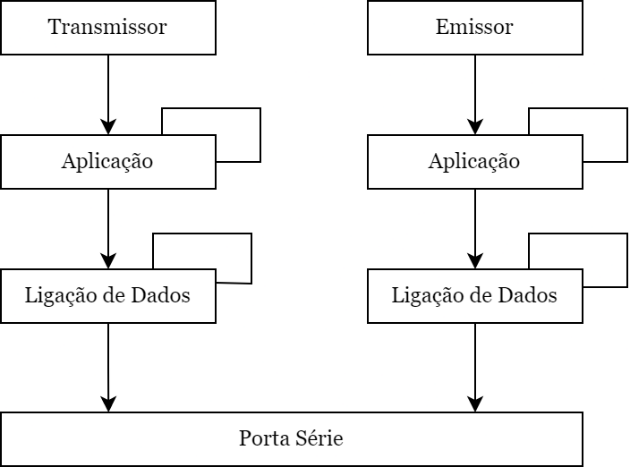
\includegraphics[width=10cm]{img/pic.png}    
    \caption{Arquitetura da aplicação}
\end{figure}

\begin{itemize}
    \item A \textbf{camada da aplicação} é a responsável leitura/criação do novo ficheiro. O comportamento desta camada tem de ser especificado para determinar o seu comportamento
    \item A \textbf{camada de ligação de dados} é a responsável tanto por ler e escrever na porta série quanto por lidar com possíveis erros na transmissão das tramas. Esta camada não tem qualquer autonomia, só realiza as ações de transmissão e emissão quando solicitada
    \item A \textbf{camada de protocolo} já está implementada e a interação é feita através de system calls
\end{itemize}
